%TCIDATA{Version=5.00.0.2606}
%TCIDATA{LaTeXparent=0,0,..\Elvira-Book.tex}
%TCIDATA{ChildDefaults=chapter:1,page:1}

\section{Introduction}

\subsection{Influence diagrams formalism}

\textit{Influence diagrams} (IDs) are a powerful tool for representing a solving
decision making problems. In these problems a decision maker faces
the necessity to decide among several alternatives. For example,
let us suppose a medical problem where the decision maker is the
doctor deciding about the tests or treatments to make.

Usually, the decision making process involves uncertainty. When a
doctor applies a treatment it is not sure the impact of such a
treatment on the patient. Without uncertainty decision making would
suppose to build a set of fixed rules, applying them when required
and without any kind of doubt.

Essentially, when a decision maker has to choose an action between a set
of alternatives it is needed to sort them according to some criteria and
selecting the most valuable one. Thus, the value of an alternative usually
includes different aspects. In medical decision making some of these
aspects could be economical cost, risk, final quality of life, etc.

Therefore, the key issues about any decision problem are the ones
described above:

\begin{itemize}
\item The \textit{decision variables} under the decision maker control. For
each decision variable the decision maker must choose an state between the
state space for that variable. For example, a decision variable for a medical
problem can be a treatment, being the alternatives (state space) for the
variable the possible treatments to apply. A decision problem may contains
only one decision variable (\textit{single stage} decision problems) or several
decision variables (\textit{multiple stage} decision problems).

\item The \textit{random variables} which the decision maker can not control. These
variables represents the uncertainty about the problem. Some examples may be the
real impact of a treatment, the reliability of a test, the aggressiveness of a virus, etc.

\item The \textit{preferences} used by the decision makers to sort the alternatives
according to its desiderability. As we have explained before, the preferences can
summarize several aspects of different nature: economical cost, risk, injuries, etc.
\end{itemize}

The main advantage of IDs is the ability to gather all of these issues on a
clear and graphical formalism. Decision variables, random variables and preferences
are directly represented within IDs. IDs are directed acyclic graphs, where decision
variables, random variables and preferences are represented as squared nodes,
circles and diamonds respectively. Every variable is represented as a node in the
graph. Nodes related to random variables are called \textit{chance} nodes; decision
nodes correspond to decision variables and \textit{value} nodes are related to
preferences. With this in mind both terms, node or variable, will be used indifferently.
The relations between the variables of the problem are captured with arcs
linking their nodes. The meaning of a link depends on its destiny:

\begin{itemize}
\item A link into a chance node represents probabilistic dependence. A link from
$A$ (chance or decision) to $B$ chance node means that the value for $B$ depends on the
value for $A$. This dependency can be quantified with a probability distribution
$P(B|A, \ldots)$. Observe that the probability distribution depends on all the nodes
with arcs towards $B$.

\item A link into a decision node means available information. Therefore, a link
from $A$ node (chance or decision) into $B$ decision node means that the
decision maker, when deciding about $B$, knows the value for $A$. That is the
reason why these links are called \textit{informatives}.

\item A link into a value node represents functional dependence. A link from $A$ node
(chance or decision) into $B$ value node means that the prefences represented by $B$
depends on the value for $A$. In this case, the function quantifying the preferences
will be like this: $B(A, \ldots)$, having as domain the set of nodes with links towards
$B$.
\end{itemize}

We can distinguish two kind of knowledge represented by and ID. The first one,
called \textit{structural or qualitative} information, points the variables taking
part into the problem, as well as the relations between them. The second one is
termed \textit{numerical or quantitative} information giving values to the dependencies
(probabilistic and functional) present in the structural level.

To clarify all of these concepts we will use a very well know ID. It represents a
problem about the construction of a reactor of advanced or conventional design (Bielza
y Shenoy, ref Graphical Asymmetric Decision Problems), see Fig. \ref{reactorID}.

\begin{figure}[h]
\begin{center}
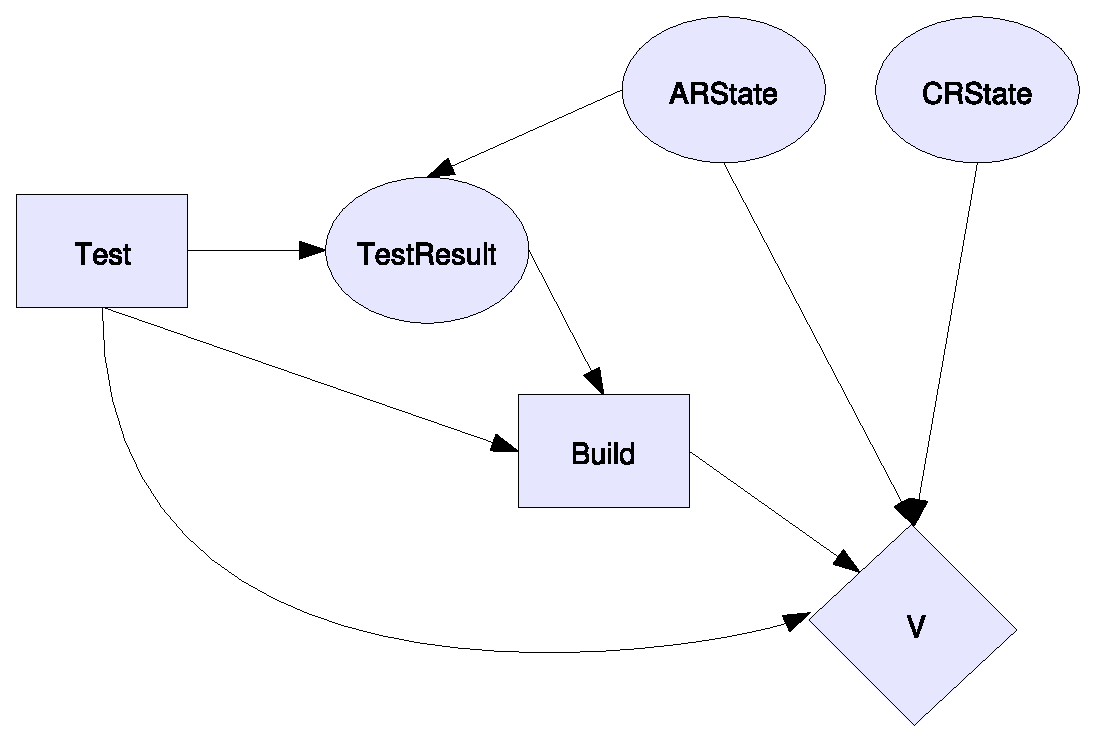
\includegraphics[scale=0.4]{./ID/fig/reactorID}
\vspace{-0.5cm}
\caption{Reactor influence diagram}
\label{reactorID}
\end{center}
\end{figure}
\vspace{-0.4cm}

This ID represents an scenario where an electric utility firm must decide whether
to build a reactor of advanced or conventional design. This decision is represented
with the node $Build$, being its state space ${advanced, \, conventional \, none}$.
Before making this decision, the company can perform a test of the components of
the advanced reactor. The election about performing the test is represented with
the node $Test$, with ${yes, no}$ as alternatives. Usually, IDs formalism assume
that the decision maker does not forget its previous decisions. With this in mind,
the \textit{informative} arc from $Test$ to $Build$ represents this situation,
called \textit{non-forgetting}. In fact,this arc could be removed without loosing
information, just because the presence of such arc is implicit to the model.

The real state of the components of both kind of reactors is represented with
the chance nodes $ARState$ (for advanced design reactor) and $CRState$ (for
conventional design reactor). An advanced reactor can be more profitable, although
it is riskier. All what is known about these components is derived from previous
experiences. Therefore, the state of the components of advanced design reactors
can produce

\begin{itemize}
\item a safe installation. This state is called $as$ (advanced safe), being its
probability 0.66
\item an installation leading to a limited accident; state $al$
(advanced limited accident), with 0.244 of probability
\item a plant where a major accident occurs; state $am$ (advanced major accident),
with 0.096 of probability
\end{itemize}

\noindent while for conventional design reactors the probalities are as follows:

\begin{itemize}
\item 0.98 of no failure (state $cs$, conventional safe)
\item 0.02 of failure (state $cf$, conventional failure)
\end{itemize}

In this problem neither $ARState$ nor $CRState$ has incoming arcs, and therefore
the probability distributions, as shown above, are $P(ARState)$ and $P(CRState)$.
$TestResult$ is another chance node representing the reliability of the test. It
depends on the real state of the advanced reactor components. The states for this
variable are: $bad$, $good$, $excellent$ and $noResult$. The likelihoods for the
test results are presented in the Table \ref{testResultProb}.

\begin{table}[h]
\begin{center}
\begin{tabular}{|c|c|c|c|c|c|c|}
\hline
$P(TestResult|Test,ARstate)$& $yes, as$ & $yes, al$ & $yes, am$ & $no, as$ & $no, al$ & $no, am$\\ \hline
$bad$  & 0 & 0.288 & 0.313 & 0 & 0 & 0\\ \hline
$good$ & 0.182 & 0.565 & 0.437 & 0 & 0 & 0\\ \hline
$excellent$ & 0.818 & 0.147 & 0.250 & 0 & 0 & 0\\ \hline
$noResults$ & 0 & 0 & 0 & 1 & 1 & 1\\ \hline
\end{tabular}
\end{center}
\vspace{-0.5cm}
\caption{$P(TestResult|ARstate)$}
\label{testResultProb}
\end{table}

Finally, the preferences for this decision are based on the expected profits:

\begin{itemize}
\item if the firm build a conventional reactor the expected profit is
about \$8B and -\$4B in case of failure
\item if the advanced reactor is built, the expected profits are: \$12B
in case of no failure, -\$6B in case of limited accident and -\$10B if
there is a major accident
\item the cost of performing the test about the state of the advanced
reactor components is \$1B
\end{itemize}

Therefore, the function representing the preferences for this decision
problem can be represented with the tree in Fig. \ref{prefTree}. As it
will be explained later these tree-style representation presents several
advantages when solving influence diagrams.

\begin{figure}[h]
\begin{center}
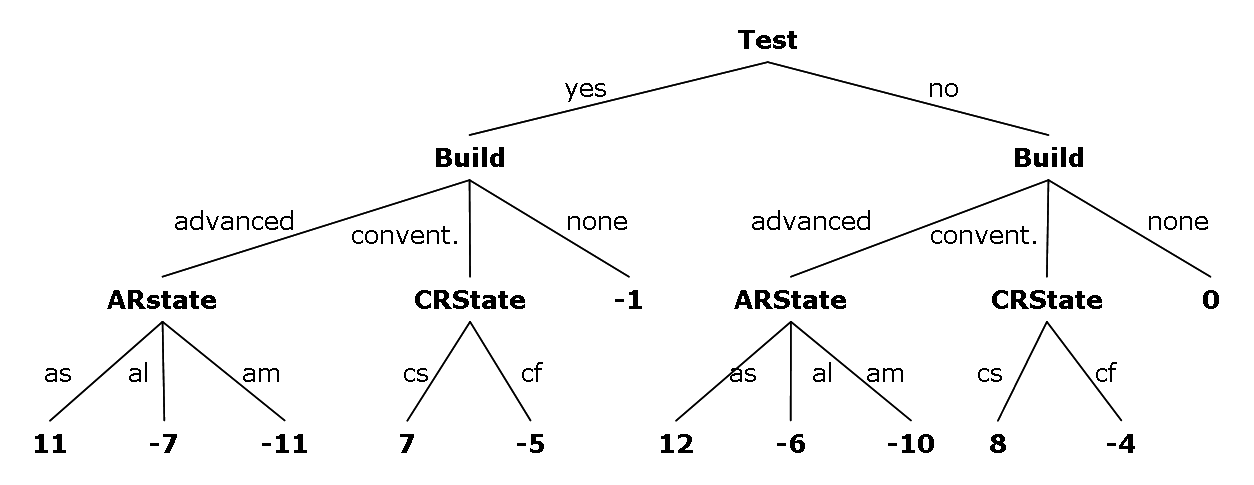
\includegraphics[scale=0.5]{./ID/fig/prefTree}
\vspace{-0.5cm}
\caption{Preferences for reactor build problem}
\label{prefTree}
\end{center}
\end{figure}

After this brief walk over the basic elements of the IDs, the next section
introduces the basic notation used throughout the rest of the chapter.

\subsection{Notation}

The set of chance nodes will be denoted $V_{C}$; the set of decision nodes
is $V_D$ and the set of utility nodes is $V_U$.  The set of nodes having $X$ as
direct successor is called $parents(X)$. The set of nodes having $X$ as direct
or indirect successor is denoted $ant(X)$. Those nodes having $X$ as parent is
termed $childs(X)$. Let $suc(X)$ be the set of nodes having $X$ as antecessor.
These sets can be particularized according to the kind of nodes they contain. For
example, $parents_{C}(X)$ denotes the set of chance nodes being parents of
$X$.

Let $\Omega_X$ be the domain for the discrete variable $X$.  The number of
states in the domain of $X$ is denoted $card(X)$. To distinguish
between variables and set of variables will denote a set of
variables $X_J=\{X_{j1},\ldots,X_{jn}\}$. Given a set $X_J$ of variables then $\Omega_{X_J}$
defines the Cartesian product for the states of the variables in $X_J$. The values belonging
to $\Omega_{X_J}$ are called \textit{configurations}. The set of variables known to the decision
maker when deciding on a given decision $D_i$ is called \textit{information predecessors}
of $D_i$ and is denoted $infPred(D_i)$. We will assume that the decision maker remembers
all previous observations and decisions. As a consequence
$infPred(D_i) \subseteq infPred(D_{i+1})$. This is a consequence of the previously
explained \textit{non-forgetting} property. The set $\Omega_{infPred(D_{i})}$ is called the \textit{information set} for $D_i$: $IS(D_{i})$.

A potential $\phi$, defined on $U_{I}$ will be a mapping $\phi: U_I \rightarrow \Reals$.
$U_{I}$ is called the \textit{domain} for the potential: $dom(\phi)=U_{I}$.
The sets of utility potentials and probability potentials are denoted $\Psi$ and $\Phi$,
respectively. A strategy is a set of decision functions $\Delta=\{\delta_{D}| D\in V_D\}$,
where $\delta_D$ is a policy given by:

\begin{equation}
\delta_D : IS(D) \rightarrow \Omega_D
\label{policy}
\end{equation}

A strategy that maximizes the expected utility is termed an \textit{optimal strategy}. Each
policy belonging to an optimal policy will be called \textit{optimal policy}. Anyway, the
concepts of policies and strategies will be explained in the next section.

\subsection{Overview about IDs evaluation}

The objective of IDs evaluation is to produce a set of decision tables, one per decision
node, containing the policy for that decision. This policy has the form showed in Eq.
\ref{policy}. Although a complete description of methods for solving IDs will be included
in another section (REF A LA SECCION) it is important to understand the structure of such
decision tables, as well as the procedure used to query them.

Let us consider the ID explained above. In this case, the evaluation of this ID will produce
two decision tables, one for $Test$ and another for $Build$. The information sets for these
decisions are: $IS(Test) = {\emptyset}$ and $IS(Build) = {TestResults,\, Test}$ (the way to
determine these set will be explained below, as a key step for the evaluation process). The
decision table for $Build$ variable is showed in Table \ref{buildTable},

\begin{table}[h]
\begin{center}
\begin{tabular}{|c|c|c|c|c|c|c|c|c|}
\hline
 &$yes,noRes.$&$no,noRes.$&$yes,bad$&$no,bad$&$yes,good$&$no.good$&$yes,exc.$&$no,exc.$\\ \hline
$none$  & 0 & -1 & -1 & 0 & -1 & 0 & -1 & 0\\ \hline
$conventional$ & 0 & 7.76 & 6.76 & 0 & 6.76 & 9 & 6.76 & 0 \\ \hline
$advanced$ & 0 & 5.496 & 4.13 & 0 & 3.45 & 0 & 5.27 & 0 \\ \hline
\end{tabular}
\end{center}
\vspace{-0.5cm}
\caption{Decision table for $Build$ decision}
\label{buildTable}
\end{table}

\noindent and the decision table for $Test$ is presented in Table \ref{testTable}.

\begin{table}[h]
\begin{center}
\begin{tabular}{|c|c|}
\hline
$yes$ & 6.76 \\ \hline
$no$  & 7.76 \\ \hline
\end{tabular}
\end{center}
\vspace{-0.5cm}
\caption{Decision table for $Test$ decision}
\label{testTable}
\end{table}

So, when a decision maker is faced with this problem, how does he proceeds? First at all,
he should look for the decision table for $Test$ and observe that the expected value for
$no$ is higher than the one for $yes$. In this case, the most valuable alternative is not
to perform the test. With this choice in mind, the next step is to consider the decision
table for $Build$. The column of interest is the second one, related to $no$ alternative
for $Test$ and being $noResults$ the state for $TestResults$, as a consequence of the
decision of not performing the test. In this column, the most valuable alternative
corresponds to $conventional$. Therefore, this should be the selected alternative for this
decision.

\subsection{IDs drawbacks}

Although IDs capture the main features of decision problems some kind of knowledge may
be impossible to include into the formalism. For example, if we consider the ID in Fig.
\ref{reactorID}, a new statal law may forbides to build an advanced reactor if the result
of the test is bad. In this case, this \textit{qualitative} knowledge about the problem
links the value of the variables $TestResult$ and $Build$. And these variables does not
take part together on the domain of any of the potentials quantifying nor the uncertainties
neither the preferences.

The constraint outlined before is a particular ocurrence of what is called \textit{assymetry}. The
usual algorithms to solve IDs are devoted to compute the strategies for \textit{symetric} IDs. An
ID is \textit{symetric} if the formulation of the decision problem as a \textit{decision tree} 
does not include branches representing non allowed scenarios. Intuitively, an ID is
\textit{assymetric} if some combinations of values for the variables of the problem are 
somehow constrained. This situation leads to two problems:

\begin{itemize}
\item First at all, it is needed to include \textit{artificial} states in the domain of the 
variables. For example, let us consider $TestResult$ variable. The natural states for this
variable are those required to define the possible situation of the reactor components:
bad, good and excellent. However, it the domain include these states only, how to represent
the situation when the test is not performed? What state should be assigned to this
variable? As it can be seen the problem arises when the combinations of values for
$Test$ and $TestResult$ are considered together. In fact, this constraint can be expressed
with a logical relation between these variables:

\begin{equation}
Test=\{no\} \Longleftrightarrow TestResult=\{noResult\}
\label{constraint}
\end{equation}

\item The qualitative knowledge about the problem produces degenerated probability
distributions. If we observe the probability distribution for $TestResult$ 
(in Table \ref{testResultProb}), we can see the last three columns present only
one non-cero value. This means that for such columns there is only one allowed
value for $TestResult$. The degenerated distributions for some combinations of
values for the variables suppose an useless effort when computing the solution to
the ID. It would be desiderable to avoid any kind of computation with them.

\item The main problem arises when the qualitative knowledge can not be included
into any of the potentials. In this case, how to use it during the computation
of the solution? If some knowledge it is not used, the final solution will not
be completely consistent with the information about the problem. For example,
looking at the decision table for $Build$ variable, the third column represents
the situation where the result of the test is $bad$. The law says that can not
be built and advanced design reactor. Therefore, the value $4.13$ should be
0. In this problem this situation does not affect the policy for the decision,
merely because the most preferred alternative is $conventional$. But may be 
problems where the policies propose actions which does not agree with the 
constraints.
\end{itemize}

Several attempts try to superate this drawbacks. A comparison of some of them
can be seen in Bielza and Shenoy, and more recents works in Nielsen, Jensen,
Shenoy, Andr�s y yo, etc. With these improvements \textit{asymmetric} IDs can 
be solved efficiently.

Another important issue about solving IDs is the size of the potentials to manage
during the computation of the decision tables. Furthermore, these tables are
enormous for problems where there is a wide set of variables influencing the decisions
variables. Must be remembered that the number of parameters to store in a decision
table is the cartesian product of the domains of the whole set of variables taking
part into the decision table. Looking at the Eq. \ref{policy}, the number of
parameters for a decision table, $param(D)$ can be expressed:

\begin{equation}
param(D)= \Omega_{D \cup IS(D)}
\label{numberOfParemeters}
\end{equation}

\noindent and may be the intermediante potentials required to compute the decision
table are bigger than the same decision table. A complex real-world problem could
lead to the evaluation be impossible, exceeding the capacity of any usual PC. Therefore, 
a good algorithm for solving IDs should be able to deal with \textit{asymmetries}, making 
the computations as economical as possible, trying to reduce the memory and storage 
requirements.

\subsection{IDs classes hierarchy}

In this section it is included a brief description about the Elvira classes related
to IDs. More details about them will be included as long as are explained the algorithms
related to IDs. 

\subsubsection{IDiagram}

This is the main class for IDs work. It derives from \textbf{Bnet}, a general class for
representing Bayesian Networks. The objective of \textbf{IDiagram} class is to offer
particular methods related to this kind of network. These methods should not depend on
any particular evaluation algorithm.

\subsubsection{ArcReversal}

This class implements \textit{arc reversal} algorithm (ref. de Shachter). This algorithm
compute the decision tables removing chance and decision variables one by one, using
\textit{arc reversal} operation when a node can not be deleted. In fact this class gives
a general frame for a family of variations using this algorithm as a base: 
\textbf{ARWithPotentialTree}, \textit{arc reversal} algorithm using \textit{numerical trees} 
(ref de Andr�s y m�a para los �rboles num�ricos) for probabilities and preferences; and
\textbf{ARWPTAndConstraints}, \textit{arc reversal} using numerical trees and taking into account
qualitative kowledge about the problem. The use of trees, as it will be explained below, may 
reduce the computational cost of the evaluation. The last variation tries to use the
qualitative knowledge about the problem to discard unnecesary computations.

\subsubsection{VariableElimination}

\textbf{VariableElimination} class offers the methods and data required to apply this
algorithm for solving IDs (ref de Shenoy). The computation goes deleting variables under 
a certain order. This algorithm has less computational requirements than arc reversal. 
However, some applications needs to compute the complete \textit{a-posteriori} 
distributions for the variables when they are removed, something that is not possible
with this algorithm. This information is specially interesting during the model construction.
As it was explained with \textbf{ArcReversal} class, \textbf{VariableElimination} is the base 
class for a family of variations about this algorithm: \textbf{VEWithPotentialTree} and \textbf{VEWPTAndConstraints}.

\subsection{QualitativeVariableElimination}

This class apply \textit{variable elimination} algorithm on an ID but without computing
the potentials derived from removing its variables. This allows to analyze the behaviour
of the algorithm without computing decision tables. With this class it is possible to
know the computational cost of evaluating an ID with this algorithm, as well as the order
use to delete the variables, the relevant variables appearing in the decision tables,
etc.

Faltan las clases de los nodos supervalor. Quiz�s tambi�n indicar algo de la clase sobre
comparaci�n de resultados de DIs. �Alguna clase m�s?
